% hdp
\lecture{The Hierarchical Dirichlet Process}{hdp}

\begin{frame}
	\frametitle{The Hierarchical DP}
	\begin{itemize}
		\item Imagine we have $>1$ related dataset to cluster, generated by the same process
		\item Fitting separate mixtures to each results in a loss of information
		\item The \ac{HDP} allows them to be analysed together with shared parameters
		\begin{itemize}
			\item e.g. datasets clustered individually but cluster parameters (e.g. means) can be \emph{shared}
			\item Analogy: The Chinese Restaurant Franchise
		\end{itemize}
	\end{itemize}
\end{frame}

\begin{frame}
	\frametitle{The Chinese Restaurant Franchise}
	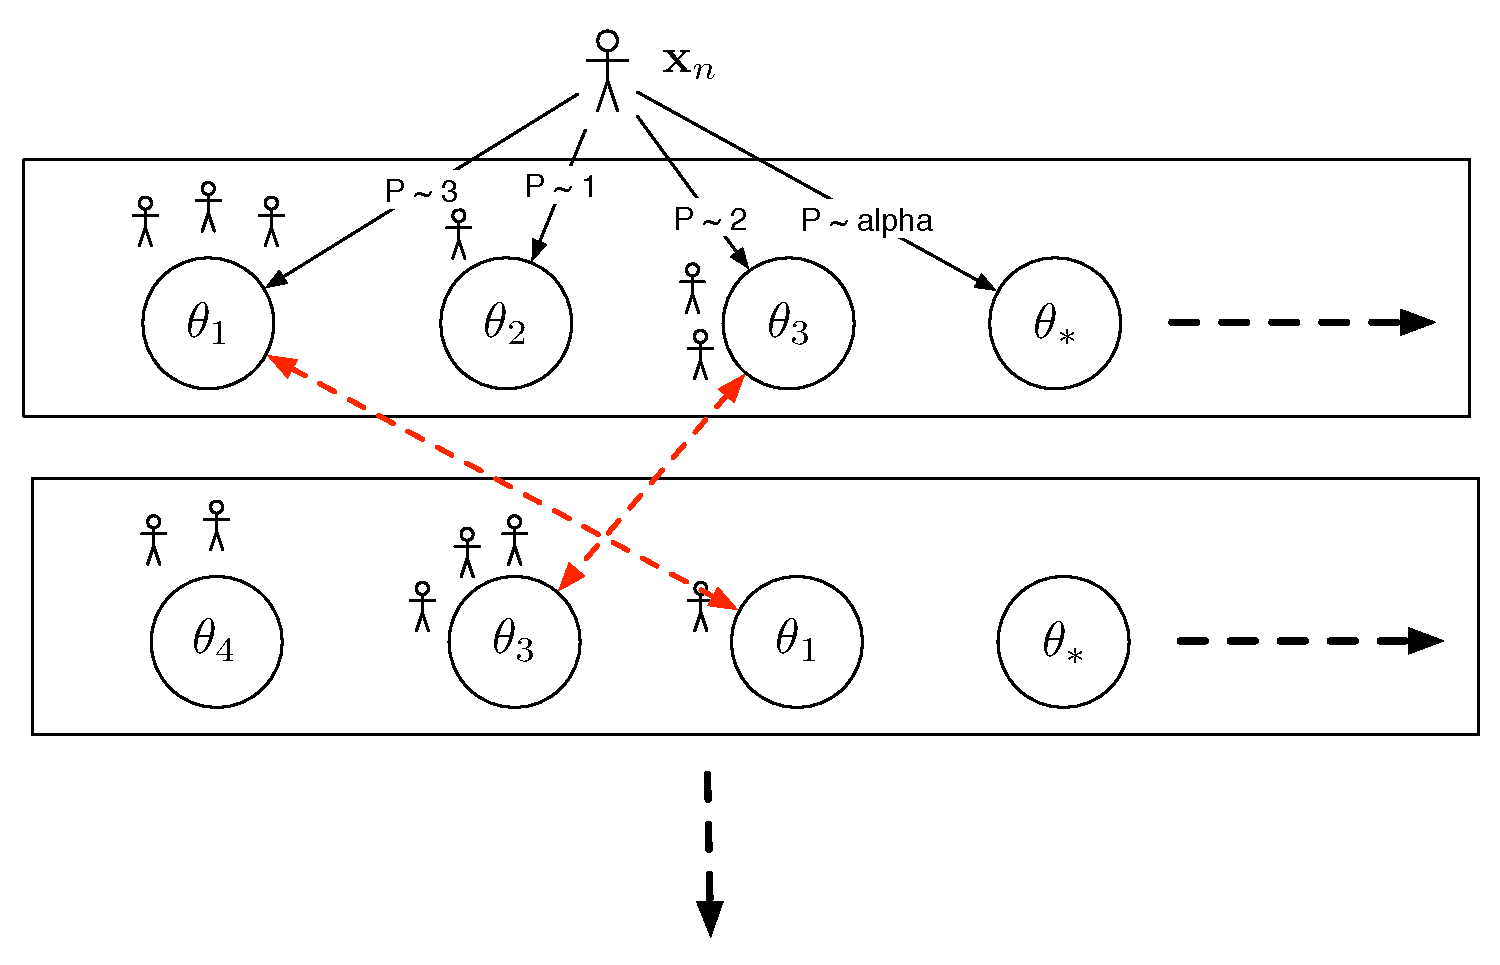
\includegraphics[width=\linewidth]{CRPfranchise}
\end{frame}

\begin{frame}
	\frametitle{The Chinese Restaurant Franchise}
	\begin{itemize}
		\item 
	\end{itemize}
\end{frame}